% Options for packages loaded elsewhere
\PassOptionsToPackage{unicode}{hyperref}
\PassOptionsToPackage{hyphens}{url}
%
\documentclass[
]{article}
\usepackage{amsmath,amssymb}
\usepackage{iftex}
\usepackage{ctex}
\ifPDFTeX
  \usepackage[T1]{fontenc}
  \usepackage[utf8]{inputenc}
  \usepackage{textcomp} % provide euro and other symbols
\else % if luatex or xetex
  \usepackage{unicode-math} % this also loads fontspec
  \defaultfontfeatures{Scale=MatchLowercase}
  \defaultfontfeatures[\rmfamily]{Ligatures=TeX,Scale=1}
\fi
\usepackage{lmodern}
\ifPDFTeX\else
  % xetex/luatex font selection
\fi
% Use upquote if available, for straight quotes in verbatim environments
\IfFileExists{upquote.sty}{\usepackage{upquote}}{}
\IfFileExists{microtype.sty}{% use microtype if available
  \usepackage[]{microtype}
  \UseMicrotypeSet[protrusion]{basicmath} % disable protrusion for tt fonts
}{}
\makeatletter
\@ifundefined{KOMAClassName}{% if non-KOMA class
  \IfFileExists{parskip.sty}{%
    \usepackage{parskip}
  }{% else
    \setlength{\parindent}{0pt}
    \setlength{\parskip}{6pt plus 2pt minus 1pt}}
}{% if KOMA class
  \KOMAoptions{parskip=half}}
\makeatother
\usepackage{xcolor}
\usepackage[margin=1in]{geometry}
\usepackage{color}
\usepackage{fancyvrb}
\newcommand{\VerbBar}{|}
\newcommand{\VERB}{\Verb[commandchars=\\\{\}]}
\DefineVerbatimEnvironment{Highlighting}{Verbatim}{commandchars=\\\{\}}
% Add ',fontsize=\small' for more characters per line
\usepackage{framed}
\definecolor{shadecolor}{RGB}{248,248,248}
\newenvironment{Shaded}{\begin{snugshade}}{\end{snugshade}}
\newcommand{\AlertTok}[1]{\textcolor[rgb]{0.94,0.16,0.16}{#1}}
\newcommand{\AnnotationTok}[1]{\textcolor[rgb]{0.56,0.35,0.01}{\textbf{\textit{#1}}}}
\newcommand{\AttributeTok}[1]{\textcolor[rgb]{0.13,0.29,0.53}{#1}}
\newcommand{\BaseNTok}[1]{\textcolor[rgb]{0.00,0.00,0.81}{#1}}
\newcommand{\BuiltInTok}[1]{#1}
\newcommand{\CharTok}[1]{\textcolor[rgb]{0.31,0.60,0.02}{#1}}
\newcommand{\CommentTok}[1]{\textcolor[rgb]{0.56,0.35,0.01}{\textit{#1}}}
\newcommand{\CommentVarTok}[1]{\textcolor[rgb]{0.56,0.35,0.01}{\textbf{\textit{#1}}}}
\newcommand{\ConstantTok}[1]{\textcolor[rgb]{0.56,0.35,0.01}{#1}}
\newcommand{\ControlFlowTok}[1]{\textcolor[rgb]{0.13,0.29,0.53}{\textbf{#1}}}
\newcommand{\DataTypeTok}[1]{\textcolor[rgb]{0.13,0.29,0.53}{#1}}
\newcommand{\DecValTok}[1]{\textcolor[rgb]{0.00,0.00,0.81}{#1}}
\newcommand{\DocumentationTok}[1]{\textcolor[rgb]{0.56,0.35,0.01}{\textbf{\textit{#1}}}}
\newcommand{\ErrorTok}[1]{\textcolor[rgb]{0.64,0.00,0.00}{\textbf{#1}}}
\newcommand{\ExtensionTok}[1]{#1}
\newcommand{\FloatTok}[1]{\textcolor[rgb]{0.00,0.00,0.81}{#1}}
\newcommand{\FunctionTok}[1]{\textcolor[rgb]{0.13,0.29,0.53}{\textbf{#1}}}
\newcommand{\ImportTok}[1]{#1}
\newcommand{\InformationTok}[1]{\textcolor[rgb]{0.56,0.35,0.01}{\textbf{\textit{#1}}}}
\newcommand{\KeywordTok}[1]{\textcolor[rgb]{0.13,0.29,0.53}{\textbf{#1}}}
\newcommand{\NormalTok}[1]{#1}
\newcommand{\OperatorTok}[1]{\textcolor[rgb]{0.81,0.36,0.00}{\textbf{#1}}}
\newcommand{\OtherTok}[1]{\textcolor[rgb]{0.56,0.35,0.01}{#1}}
\newcommand{\PreprocessorTok}[1]{\textcolor[rgb]{0.56,0.35,0.01}{\textit{#1}}}
\newcommand{\RegionMarkerTok}[1]{#1}
\newcommand{\SpecialCharTok}[1]{\textcolor[rgb]{0.81,0.36,0.00}{\textbf{#1}}}
\newcommand{\SpecialStringTok}[1]{\textcolor[rgb]{0.31,0.60,0.02}{#1}}
\newcommand{\StringTok}[1]{\textcolor[rgb]{0.31,0.60,0.02}{#1}}
\newcommand{\VariableTok}[1]{\textcolor[rgb]{0.00,0.00,0.00}{#1}}
\newcommand{\VerbatimStringTok}[1]{\textcolor[rgb]{0.31,0.60,0.02}{#1}}
\newcommand{\WarningTok}[1]{\textcolor[rgb]{0.56,0.35,0.01}{\textbf{\textit{#1}}}}
\usepackage{longtable,booktabs,array}
\usepackage{calc} % for calculating minipage widths
% Correct order of tables after \paragraph or \subparagraph
\usepackage{etoolbox}
\makeatletter
\patchcmd\longtable{\par}{\if@noskipsec\mbox{}\fi\par}{}{}
\makeatother
% Allow footnotes in longtable head/foot
\IfFileExists{footnotehyper.sty}{\usepackage{footnotehyper}}{\usepackage{footnote}}
\makesavenoteenv{longtable}
\usepackage{graphicx}
\makeatletter
\def\maxwidth{\ifdim\Gin@nat@width>\linewidth\linewidth\else\Gin@nat@width\fi}
\def\maxheight{\ifdim\Gin@nat@height>\textheight\textheight\else\Gin@nat@height\fi}
\makeatother
% Scale images if necessary, so that they will not overflow the page
% margins by default, and it is still possible to overwrite the defaults
% using explicit options in \includegraphics[width, height, ...]{}
\setkeys{Gin}{width=\maxwidth,height=\maxheight,keepaspectratio}
% Set default figure placement to htbp
\makeatletter
\def\fps@figure{htbp}
\makeatother
\setlength{\emergencystretch}{3em} % prevent overfull lines
\providecommand{\tightlist}{%
  \setlength{\itemsep}{0pt}\setlength{\parskip}{0pt}}
\setcounter{secnumdepth}{-\maxdimen} % remove section numbering
\ifLuaTeX
  \usepackage{selnolig}  % disable illegal ligatures
\fi
\usepackage{bookmark}
\IfFileExists{xurl.sty}{\usepackage{xurl}}{} % add URL line breaks if available
\urlstyle{same}
\hypersetup{
  pdftitle={地理建模实验6 实验报告},
  pdfauthor={42109232 \quad 吕文博 \quad 地信2101班},
  hidelinks,
  pdfcreator={LaTeX via pandoc}}

\title{地理建模实验6 实验报告}
\author{42109232 \quad 吕文博 \quad 地信2101班}
\date{2024-06-11}

\begin{document}
\maketitle

\subsection{主成分分析}\label{ux4e3bux6210ux5206ux5206ux6790}

\subsubsection{读取和清洗数据}\label{ux8bfbux53d6ux548cux6e05ux6d17ux6570ux636e}

\begin{Shaded}
\begin{Highlighting}[]
\FunctionTok{library}\NormalTok{(tidyverse)}
\FunctionTok{library}\NormalTok{(broom)}
\FunctionTok{library}\NormalTok{(ggfortify)}
\NormalTok{urban\_econindic }\OtherTok{=}\NormalTok{ readxl}\SpecialCharTok{::}\FunctionTok{read\_xlsx}\NormalTok{(}\StringTok{\textquotesingle{}../data/exp6/6.xlsx\textquotesingle{}}\NormalTok{,}\AttributeTok{sheet =} \StringTok{\textquotesingle{}Chp第16题\textquotesingle{}}\NormalTok{)}
\FunctionTok{names}\NormalTok{(urban\_econindic) }\OtherTok{=} \FunctionTok{str\_extract}\NormalTok{(}\FunctionTok{names}\NormalTok{(urban\_econindic),}\StringTok{"\^{}[\^{}/]+"}\NormalTok{)}
\FunctionTok{head}\NormalTok{(urban\_econindic) }\SpecialCharTok{\%\textgreater{}\%}\NormalTok{ knitr}\SpecialCharTok{::}\FunctionTok{kable}\NormalTok{()}
\end{Highlighting}
\end{Shaded}

\begin{longtable}[]{@{}
  >{\raggedleft\arraybackslash}p{(\columnwidth - 14\tabcolsep) * \real{0.0811}}
  >{\raggedleft\arraybackslash}p{(\columnwidth - 14\tabcolsep) * \real{0.0721}}
  >{\raggedleft\arraybackslash}p{(\columnwidth - 14\tabcolsep) * \real{0.1351}}
  >{\raggedleft\arraybackslash}p{(\columnwidth - 14\tabcolsep) * \real{0.0991}}
  >{\raggedleft\arraybackslash}p{(\columnwidth - 14\tabcolsep) * \real{0.0991}}
  >{\raggedleft\arraybackslash}p{(\columnwidth - 14\tabcolsep) * \real{0.1712}}
  >{\raggedleft\arraybackslash}p{(\columnwidth - 14\tabcolsep) * \real{0.1892}}
  >{\raggedleft\arraybackslash}p{(\columnwidth - 14\tabcolsep) * \real{0.1532}}@{}}
\toprule\noalign{}
\begin{minipage}[b]{\linewidth}\raggedleft
城市编号
\end{minipage} & \begin{minipage}[b]{\linewidth}\raggedleft
总人口
\end{minipage} & \begin{minipage}[b]{\linewidth}\raggedleft
非农业人口比例
\end{minipage} & \begin{minipage}[b]{\linewidth}\raggedleft
农业总产值
\end{minipage} & \begin{minipage}[b]{\linewidth}\raggedleft
工业总产值
\end{minipage} & \begin{minipage}[b]{\linewidth}\raggedleft
地方财政预算内收入
\end{minipage} & \begin{minipage}[b]{\linewidth}\raggedleft
城乡居民年底储蓄余额
\end{minipage} & \begin{minipage}[b]{\linewidth}\raggedleft
在岗职工工资总额
\end{minipage} \\
\midrule\noalign{}
\endhead
\bottomrule\noalign{}
\endlastfoot
1 & 1249.90 & 0.60 & 184.34 & 1999.97 & 279.09 & 2680.66 & 577.33 \\
2 & 910.17 & 0.58 & 150.11 & 2264.55 & 112.81 & 1130.19 & 225.43 \\
3 & 875.40 & 0.23 & 291.87 & 688.58 & 35.23 & 709.59 & 75.89 \\
4 & 299.92 & 0.66 & 23.60 & 273.78 & 20.33 & 394.31 & 65.40 \\
5 & 207.78 & 0.44 & 36.53 & 81.65 & 10.58 & 139.66 & 30.93 \\
6 & 677.08 & 0.63 & 129.54 & 582.67 & 56.79 & 901.70 & 115.28 \\
\end{longtable}

\subsubsection{\texorpdfstring{使用baseR的\texttt{prcomp}函数联同\texttt{tidyverse}执行主成分分析}{使用baseR的prcomp函数联同tidyverse执行主成分分析}}\label{ux4f7fux7528baserux7684prcompux51fdux6570ux8054ux540ctidyverseux6267ux884cux4e3bux6210ux5206ux5206ux6790}

\begin{Shaded}
\begin{Highlighting}[]
\NormalTok{urban\_econpca }\OtherTok{=}\NormalTok{ urban\_econindic }\SpecialCharTok{\%\textgreater{}\%} 
  \FunctionTok{nest}\NormalTok{() }\SpecialCharTok{\%\textgreater{}\%} 
  \FunctionTok{mutate}\NormalTok{(}\AttributeTok{pca =} \FunctionTok{map}\NormalTok{(data, \textbackslash{}(x) }\FunctionTok{prcomp}\NormalTok{(}\FunctionTok{select}\NormalTok{(x,}\SpecialCharTok{{-}}\StringTok{\textasciigrave{}}\AttributeTok{城市编号}\StringTok{\textasciigrave{}}\NormalTok{),}
                                     \AttributeTok{center =} \ConstantTok{TRUE}\NormalTok{, }\AttributeTok{scale =} \ConstantTok{TRUE}\NormalTok{)),}
         \AttributeTok{pca\_aug =} \FunctionTok{map2}\NormalTok{(pca, data, \textbackslash{}(x,y) }\FunctionTok{augment}\NormalTok{(x, }\AttributeTok{data =}\NormalTok{ y)))}

\NormalTok{urban\_econpca}
\end{Highlighting}
\end{Shaded}

\begin{verbatim}
## # A tibble: 1 x 3
##   data              pca      pca_aug           
##   <list>            <list>   <list>            
## 1 <tibble [35 x 8]> <prcomp> <tibble [35 x 16]>
\end{verbatim}

\begin{Shaded}
\begin{Highlighting}[]
\NormalTok{var\_exp }\OtherTok{=}\NormalTok{ urban\_econpca }\SpecialCharTok{\%\textgreater{}\%} 
  \FunctionTok{unnest}\NormalTok{(pca\_aug) }\SpecialCharTok{\%\textgreater{}\%} 
  \FunctionTok{summarise}\NormalTok{(}\FunctionTok{across}\NormalTok{(}\FunctionTok{contains}\NormalTok{(}\StringTok{".fittedPC"}\NormalTok{),\textbackslash{}(x) stats}\SpecialCharTok{::}\FunctionTok{var}\NormalTok{(x))) }\SpecialCharTok{\%\textgreater{}\%} 
  \FunctionTok{gather}\NormalTok{(}\AttributeTok{key =}\NormalTok{ pc, }\AttributeTok{value =}\NormalTok{ variance) }\SpecialCharTok{\%\textgreater{}\%} 
  \FunctionTok{mutate}\NormalTok{(}\AttributeTok{var\_exp =}\NormalTok{ variance }\SpecialCharTok{/} \FunctionTok{sum}\NormalTok{(variance),}
         \AttributeTok{cum\_var\_exp =} \FunctionTok{cumsum}\NormalTok{(var\_exp),}
         \AttributeTok{pc =} \FunctionTok{str\_replace}\NormalTok{(pc, }\StringTok{".fitted"}\NormalTok{, }\StringTok{""}\NormalTok{))}

\NormalTok{var\_exp}
\end{Highlighting}
\end{Shaded}

\begin{verbatim}
## # A tibble: 7 x 4
##   pc    variance var_exp cum_var_exp
##   <chr>    <dbl>   <dbl>       <dbl>
## 1 PC1     4.31   0.616         0.616
## 2 PC2     1.95   0.279         0.896
## 3 PC3     0.360  0.0514        0.947
## 4 PC4     0.185  0.0264        0.973
## 5 PC5     0.138  0.0198        0.993
## 6 PC6     0.0331 0.00473       0.998
## 7 PC7     0.0150 0.00214       1
\end{verbatim}

\textbf{按照特征值大于1的原则,第1主成分的初始特征值为4.31,第2主成分的初始特征值为1.95.从第
3主成分开始,其初始特征值均小于1.因此,选择前2个主成分可以得到\(89.6\%\)
的累计贡献率,即表示前2个主成分可以解释\(89.6\%\) 的总方差.}

\subsubsection{碎石图}\label{ux788eux77f3ux56fe}

\begin{Shaded}
\begin{Highlighting}[]
\NormalTok{var\_exp }\SpecialCharTok{\%\textgreater{}\%} 
  \FunctionTok{rename}\NormalTok{(}\StringTok{\textasciigrave{}}\AttributeTok{Variance Explained}\StringTok{\textasciigrave{}} \OtherTok{=}\NormalTok{ var\_exp,}
         \StringTok{\textasciigrave{}}\AttributeTok{Cumulative Variance Explained}\StringTok{\textasciigrave{}} \OtherTok{=}\NormalTok{ cum\_var\_exp) }\SpecialCharTok{\%\textgreater{}\%} 
  \FunctionTok{gather}\NormalTok{(}\AttributeTok{key =}\NormalTok{ key, }\AttributeTok{value =}\NormalTok{ value, }\StringTok{\textasciigrave{}}\AttributeTok{Variance Explained}\StringTok{\textasciigrave{}}\SpecialCharTok{:}\StringTok{\textasciigrave{}}\AttributeTok{Cumulative Variance Explained}\StringTok{\textasciigrave{}}\NormalTok{) }\SpecialCharTok{\%\textgreater{}\%} 
  \FunctionTok{ggplot}\NormalTok{(}\FunctionTok{aes}\NormalTok{(pc, value, }\AttributeTok{group =}\NormalTok{ key)) }\SpecialCharTok{+} 
  \FunctionTok{geom\_point}\NormalTok{() }\SpecialCharTok{+} 
  \FunctionTok{geom\_line}\NormalTok{() }\SpecialCharTok{+} 
  \FunctionTok{facet\_wrap}\NormalTok{(}\SpecialCharTok{\textasciitilde{}}\NormalTok{key, }\AttributeTok{scales =} \StringTok{"free\_y"}\NormalTok{) }\SpecialCharTok{+}
  \FunctionTok{theme\_bw}\NormalTok{() }\SpecialCharTok{+}
  \FunctionTok{lims}\NormalTok{(}\AttributeTok{y =} \FunctionTok{c}\NormalTok{(}\DecValTok{0}\NormalTok{, }\DecValTok{1}\NormalTok{)) }\SpecialCharTok{+}
  \FunctionTok{labs}\NormalTok{(}\AttributeTok{y =} \StringTok{"Variance"}\NormalTok{,}
       \AttributeTok{title =} \StringTok{"Variance explained by each principal component"}\NormalTok{)}
\end{Highlighting}
\end{Shaded}

\begin{center}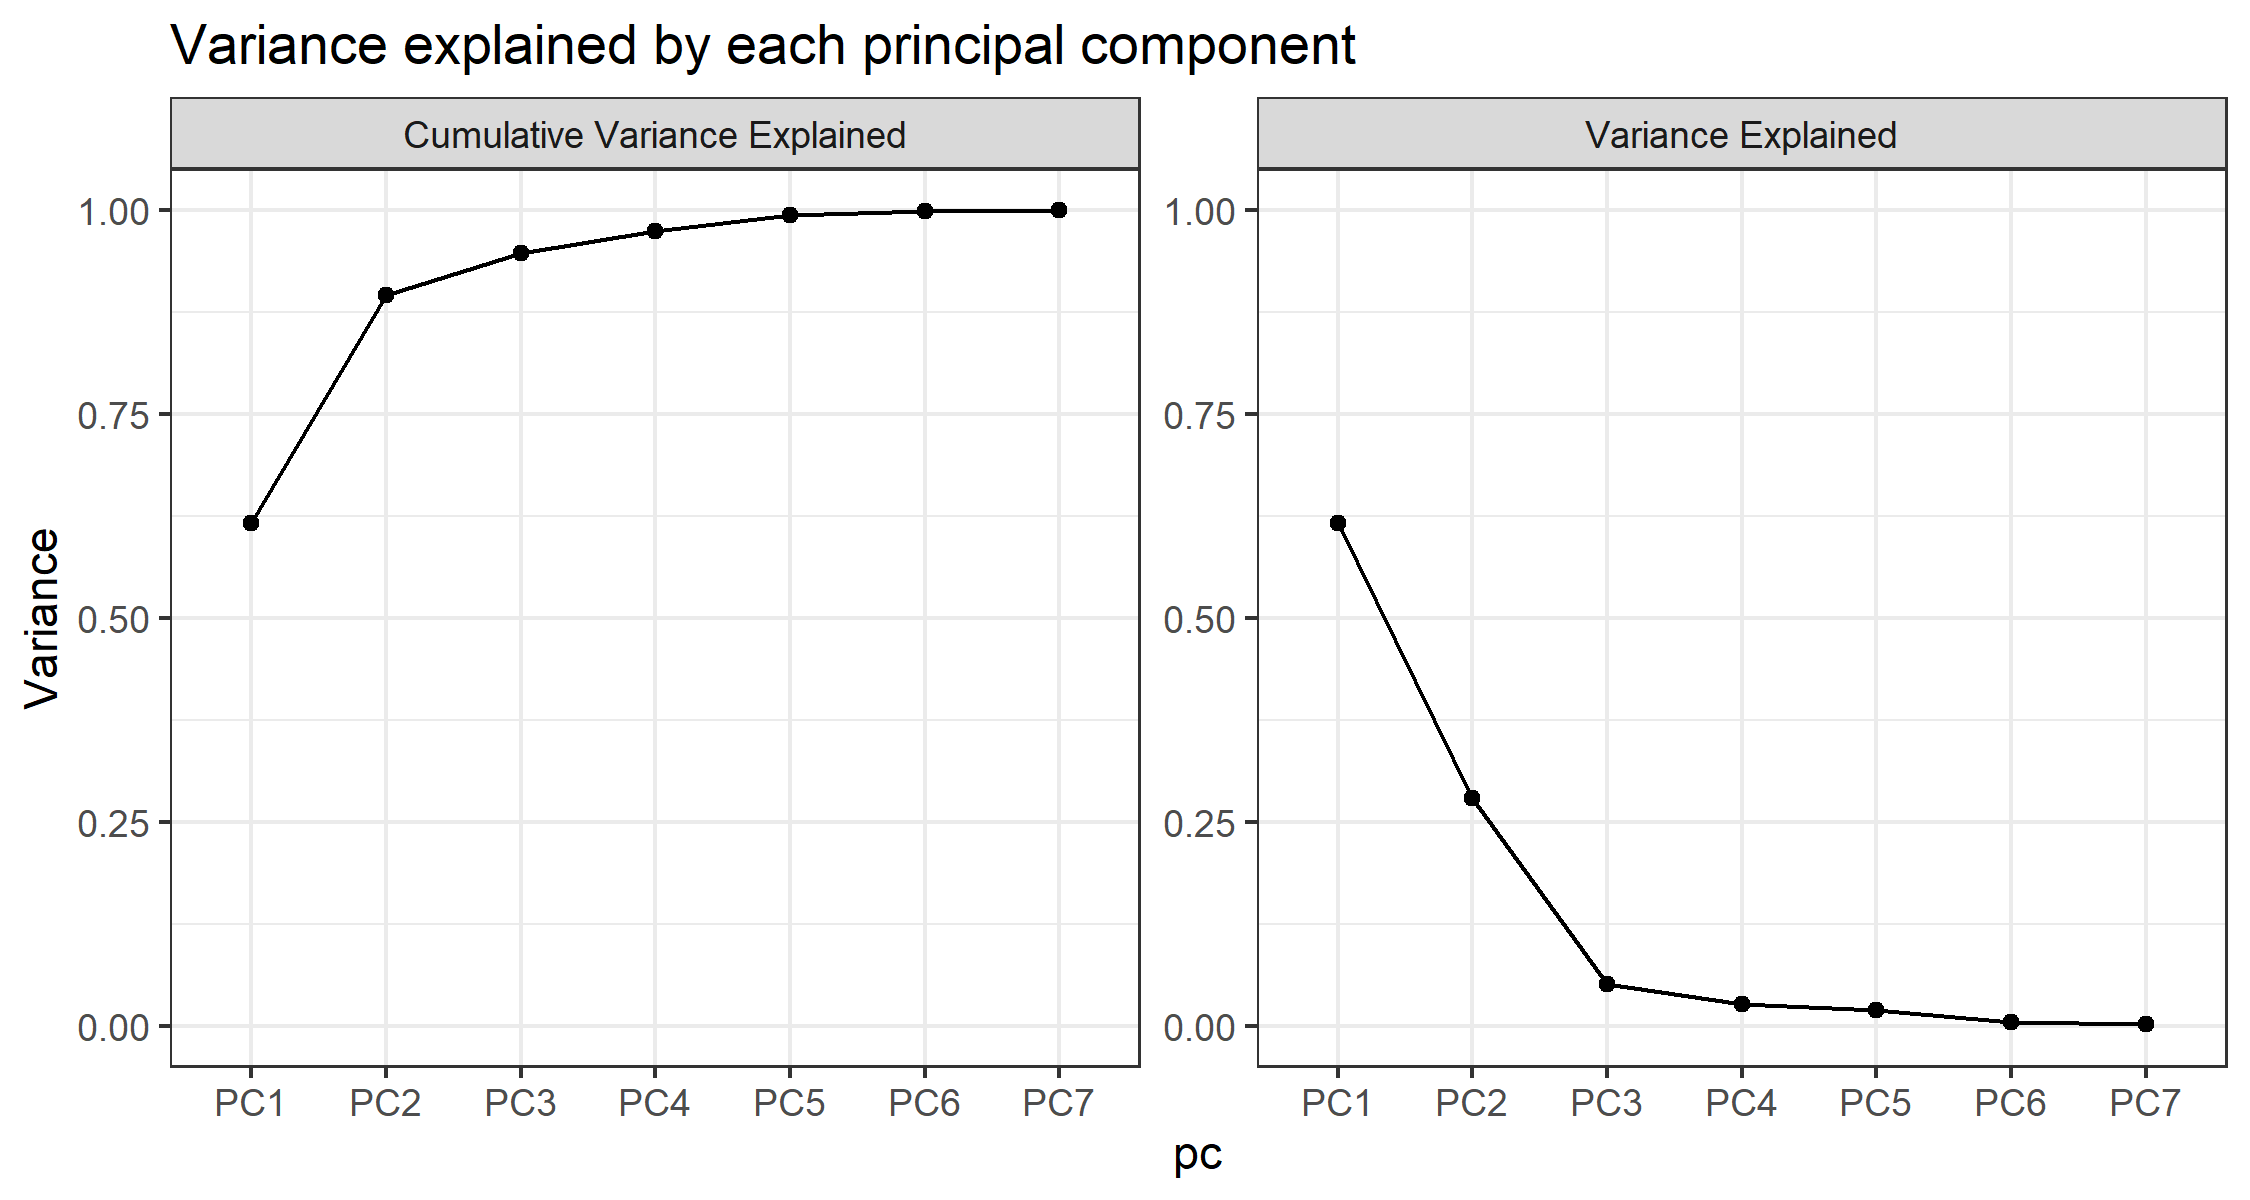
\includegraphics[width=1\linewidth,height=1\textheight]{../picture/rmd/exp6/pac_plot1-1.png} \end{center}

\textbf{从碎石图中可以看出,从第3个组件开始,特征值就处于一个较低的水平.因此选择前2
个主成分是科学的。}

\subsubsection{\texorpdfstring{将前两个主成分为\texttt{x}和\texttt{y}轴展示数据}{将前两个主成分为x和y轴展示数据}}\label{ux5c06ux524dux4e24ux4e2aux4e3bux6210ux5206ux4e3axux548cyux8f74ux5c55ux793aux6570ux636e}

\begin{Shaded}
\begin{Highlighting}[]
\NormalTok{urban\_econpca }\SpecialCharTok{\%\textgreater{}\%}
  \FunctionTok{mutate}\NormalTok{(}
    \AttributeTok{pca\_graph =} \FunctionTok{map2}\NormalTok{(}
      \AttributeTok{.x =}\NormalTok{ pca,}
      \AttributeTok{.y =}\NormalTok{ data,}
      \SpecialCharTok{\textasciitilde{}} \FunctionTok{autoplot}\NormalTok{(.x, }\AttributeTok{loadings =} \ConstantTok{TRUE}\NormalTok{, }\AttributeTok{loadings.label =} \ConstantTok{TRUE}\NormalTok{,}
                 \AttributeTok{loadings.label.repel =} \ConstantTok{TRUE}\NormalTok{,}
                 \AttributeTok{data =}\NormalTok{ .y, }\AttributeTok{label =} \ConstantTok{TRUE}\NormalTok{,}
                 \AttributeTok{label.label =} \StringTok{"城市编号"}\NormalTok{,}
                 \AttributeTok{label.repel =} \ConstantTok{TRUE}\NormalTok{) }\SpecialCharTok{+}
        \FunctionTok{theme\_bw}\NormalTok{() }\SpecialCharTok{+}
        \FunctionTok{theme}\NormalTok{(pan)}
        \FunctionTok{labs}\NormalTok{(}\AttributeTok{x =} \StringTok{"Principal Component 1"}\NormalTok{,}
             \AttributeTok{y =} \StringTok{"Principal Component 2"}\NormalTok{,}
             \AttributeTok{title =} \StringTok{"First two principal components of PCA on Urban economic indicators"}\NormalTok{)}
\NormalTok{      )}
\NormalTok{  ) }\SpecialCharTok{\%\textgreater{}\%}
  \FunctionTok{pull}\NormalTok{(pca\_graph)}
\end{Highlighting}
\end{Shaded}

\begin{center}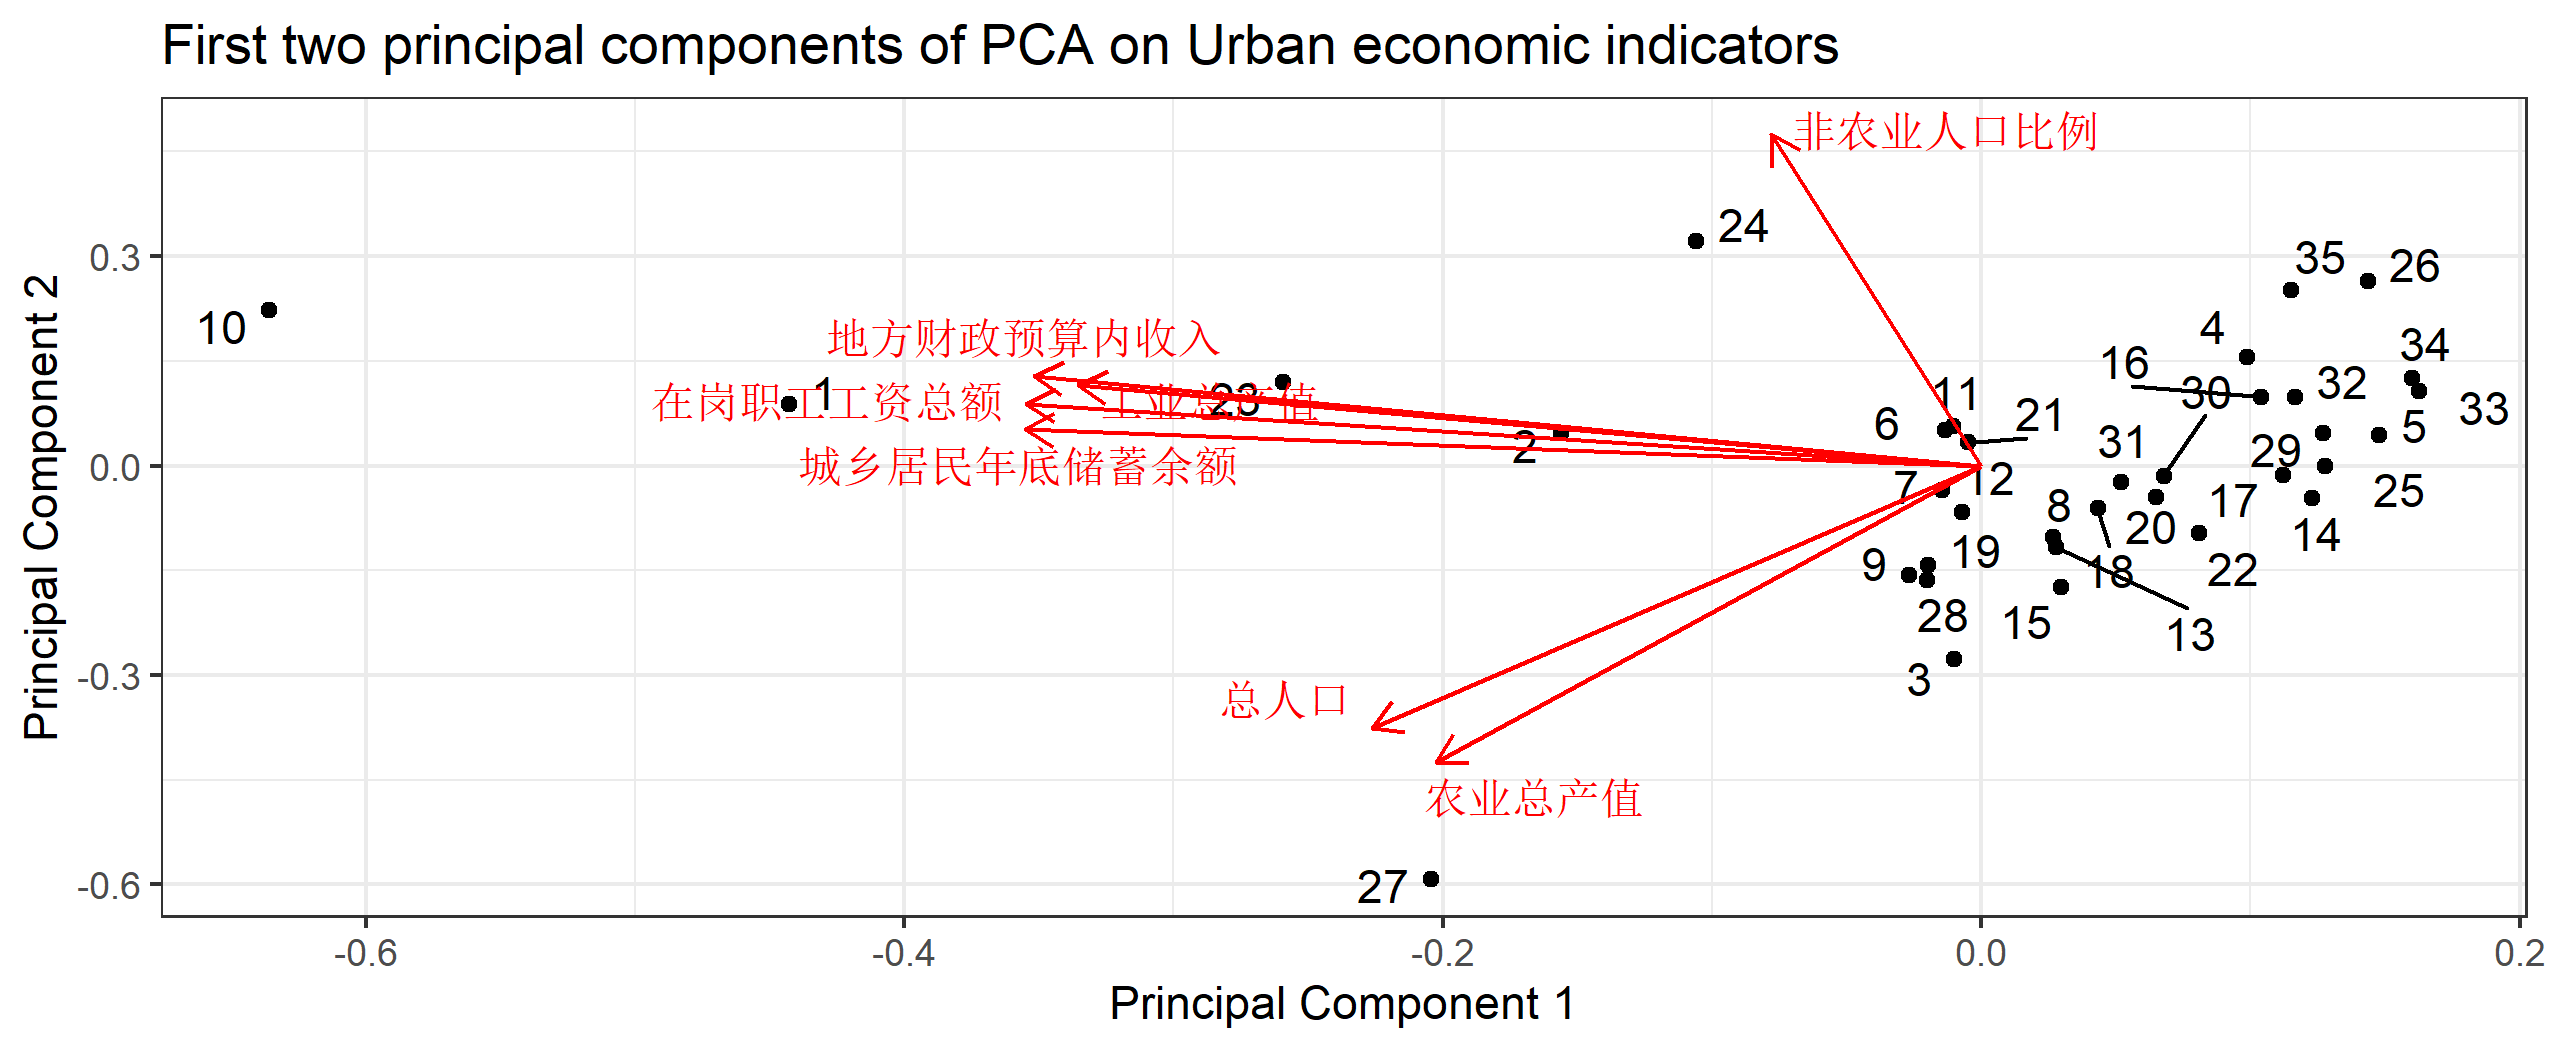
\includegraphics[width=1\linewidth,height=1\textheight]{../picture/rmd/exp6/pac_plot2-1.png} \end{center}

\subsubsection{计算综合评价得分}\label{ux8ba1ux7b97ux7efcux5408ux8bc4ux4ef7ux5f97ux5206}

R 中的特征向量默认指向负方向,因此我们将乘以 -1 来反转主成分得分的符号.

\begin{Shaded}
\begin{Highlighting}[]
\NormalTok{weight\_pca }\OtherTok{=}\NormalTok{ var\_exp }\SpecialCharTok{\%\textgreater{}\%} 
\NormalTok{  dplyr}\SpecialCharTok{::}\FunctionTok{filter}\NormalTok{(pc }\SpecialCharTok{\%in\%} \FunctionTok{c}\NormalTok{(}\StringTok{"PC1"}\NormalTok{,}\StringTok{"PC2"}\NormalTok{)) }\SpecialCharTok{\%\textgreater{}\%} 
  \FunctionTok{pull}\NormalTok{(variance) }\SpecialCharTok{\%\textgreater{}\%} 
\NormalTok{  \{. }\SpecialCharTok{/} \FunctionTok{sum}\NormalTok{(.)\}}
\NormalTok{weight\_pca}
\end{Highlighting}
\end{Shaded}

\begin{verbatim}
## [1] 0.6882711 0.3117289
\end{verbatim}

\begin{Shaded}
\begin{Highlighting}[]
\NormalTok{urban\_rank }\OtherTok{=}\NormalTok{ urban\_econpca }\SpecialCharTok{\%\textgreater{}\%} 
  \FunctionTok{unnest}\NormalTok{(pca\_aug) }\SpecialCharTok{\%\textgreater{}\%} 
  \FunctionTok{select}\NormalTok{(城市编号,}\FunctionTok{num\_range}\NormalTok{(}\StringTok{".fittedPC"}\NormalTok{,}\DecValTok{1}\SpecialCharTok{:}\DecValTok{2}\NormalTok{)) }\SpecialCharTok{\%\textgreater{}\%} 
  \FunctionTok{mutate}\NormalTok{(}\FunctionTok{across}\NormalTok{(}\SpecialCharTok{{-}}\NormalTok{城市编号,\textbackslash{}(x) }\SpecialCharTok{{-}}\NormalTok{x)) }\SpecialCharTok{\%\textgreater{}\%} 
  \FunctionTok{mutate}\NormalTok{(综合得分 }\OtherTok{=}\NormalTok{ weight\_pca[}\DecValTok{1}\NormalTok{] }\SpecialCharTok{*}\NormalTok{ .fittedPC1 }\SpecialCharTok{+}\NormalTok{ weight\_pca[}\DecValTok{2}\NormalTok{] }\SpecialCharTok{*}\NormalTok{ .fittedPC2) }\SpecialCharTok{\%\textgreater{}\%} 
  \FunctionTok{mutate}\NormalTok{(综合排名 }\OtherTok{=} \FunctionTok{min\_rank}\NormalTok{(}\FunctionTok{desc}\NormalTok{(综合得分))) }\SpecialCharTok{\%\textgreater{}\%} 
  \FunctionTok{select}\NormalTok{(城市编号,综合得分,综合排名) }\SpecialCharTok{\%\textgreater{}\%} 
  \FunctionTok{arrange}\NormalTok{(综合排名)}
\end{Highlighting}
\end{Shaded}

\textbf{注:
与SPSS结果计算有出入,SPSS中通过因子分析和综合得分两步得出结果,R直接可以运行主成分分析,R计算结果较准确}

\paragraph{城市综合排名}\label{ux57ceux5e02ux7efcux5408ux6392ux540d}

\begin{Shaded}
\begin{Highlighting}[]
\NormalTok{knitr}\SpecialCharTok{::}\FunctionTok{kable}\NormalTok{(urban\_rank)}
\end{Highlighting}
\end{Shaded}

\begin{longtable}[]{@{}rrr@{}}
\toprule\noalign{}
城市编号 & 综合得分 & 综合排名 \\
\midrule\noalign{}
\endhead
\bottomrule\noalign{}
\endlastfoot
10 & 4.8032455 & 1 \\
1 & 3.5177835 & 2 \\
27 & 3.2554747 & 3 \\
23 & 1.8837192 & 4 \\
2 & 1.2007658 & 5 \\
3 & 0.7998288 & 6 \\
9 & 0.6319004 & 7 \\
28 & 0.5925233 & 8 \\
19 & 0.5331693 & 9 \\
12 & 0.2330736 & 10 \\
7 & 0.2131860 & 11 \\
15 & 0.1980604 & 12 \\
13 & 0.0661563 & 13 \\
24 & 0.0650758 & 14 \\
8 & 0.0396344 & 15 \\
6 & -0.0191400 & 16 \\
21 & -0.0454772 & 17 \\
11 & -0.0561301 & 18 \\
18 & -0.2079732 & 19 \\
31 & -0.3791397 & 20 \\
20 & -0.4330530 & 21 \\
22 & -0.4339440 & 22 \\
30 & -0.5374285 & 23 \\
17 & -0.9126734 & 24 \\
14 & -0.9188985 & 25 \\
25 & -1.0809321 & 26 \\
16 & -1.1324317 & 27 \\
29 & -1.1946543 & 28 \\
4 & -1.2361824 & 29 \\
32 & -1.2370102 & 30 \\
5 & -1.3626954 & 31 \\
35 & -1.6209127 & 32 \\
33 & -1.6502416 & 33 \\
34 & -1.6779540 & 34 \\
26 & -1.8967252 & 35 \\
\end{longtable}

\paragraph{综合实力前五城市}\label{ux7efcux5408ux5b9eux529bux524dux4e94ux57ceux5e02}

\begin{Shaded}
\begin{Highlighting}[]
\NormalTok{urban\_rank }\SpecialCharTok{\%\textgreater{}\%} 
  \FunctionTok{head}\NormalTok{(}\DecValTok{5}\NormalTok{) }\SpecialCharTok{\%\textgreater{}\%} 
\NormalTok{  knitr}\SpecialCharTok{::}\FunctionTok{kable}\NormalTok{()}
\end{Highlighting}
\end{Shaded}

\begin{longtable}[]{@{}rrr@{}}
\toprule\noalign{}
城市编号 & 综合得分 & 综合排名 \\
\midrule\noalign{}
\endhead
\bottomrule\noalign{}
\endlastfoot
10 & 4.803246 & 1 \\
1 & 3.517784 & 2 \\
27 & 3.255475 & 3 \\
23 & 1.883719 & 4 \\
2 & 1.200766 & 5 \\
\end{longtable}

\paragraph{综合实力后五城市}\label{ux7efcux5408ux5b9eux529bux540eux4e94ux57ceux5e02}

\begin{Shaded}
\begin{Highlighting}[]
\NormalTok{urban\_rank }\SpecialCharTok{\%\textgreater{}\%} 
  \FunctionTok{tail}\NormalTok{(}\DecValTok{5}\NormalTok{) }\SpecialCharTok{\%\textgreater{}\%} 
\NormalTok{  knitr}\SpecialCharTok{::}\FunctionTok{kable}\NormalTok{()}
\end{Highlighting}
\end{Shaded}

\begin{longtable}[]{@{}rrr@{}}
\toprule\noalign{}
城市编号 & 综合得分 & 综合排名 \\
\midrule\noalign{}
\endhead
\bottomrule\noalign{}
\endlastfoot
5 & -1.362695 & 31 \\
35 & -1.620913 & 32 \\
33 & -1.650242 & 33 \\
34 & -1.677954 & 34 \\
26 & -1.896725 & 35 \\
\end{longtable}

\end{document}
